\section{改变物体热能的方法}\label{sec:5-4}

用什么方法可以改变物体的热能呢?

用热传递的办法来改变物体的热能,这是大家都熟悉的。
在热传递的过程中,一个物体吸收了热量,温度升高,它的热能就增加。
反过来,         一个物体放出了热量,温度降低,它的热能就减少。

除了热传递,用做功的办法也可以改变物体的热能。

\begin{figure}[htbp]
    \centering
    \begin{minipage}{9cm}
    \centering
    \vspace{2cm}
    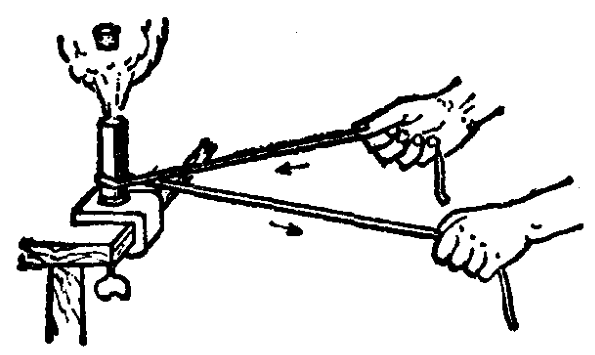
\includegraphics[width=8cm]{../pic/czwl2-ch5-4}
    \caption{克服摩擦做功使物体的热能增加}\label{fig:5-4}
    \end{minipage}
    \qquad
    \begin{minipage}{5cm}
    \centering
    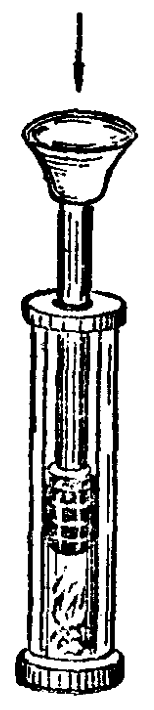
\includegraphics[width=1.5cm]{../pic/czwl2-ch5-5}
    \caption{压缩气体做功使物体的热能增加}\label{fig:5-5}
    \end{minipage}
\end{figure}

如图 \ref{fig:5-4} 所示,把一个薄壁金属管固定在支座上,管里装一些乙醚,然后用塞子塞紧。
把一根绳子缠在管子上,并迅速地来回拉绳子。过一会儿乙醚会沸腾,乙醚蒸气会把塞子冲开。
乙醚的温度升高,甚至达到了沸腾,说明它的热能增加了。
乙醚的热能增加,是因为克服绳子和管壁之间的摩擦做功而引起的。
我们通常说的摩擦生热,都是指的这类现象,即克服摩擦做功使物体的热能增加。

\begin{wrapfigure}{r}{6cm}
    \centering
    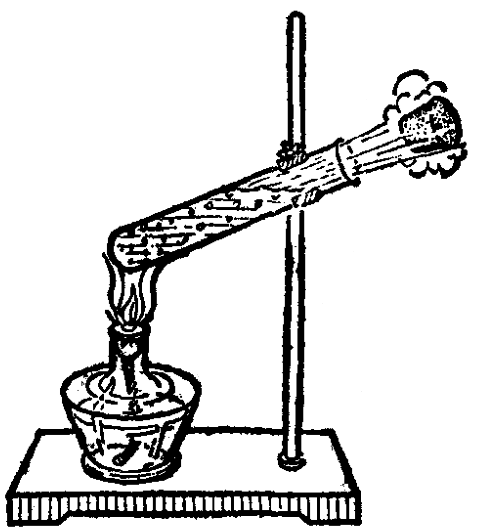
\includegraphics[width=5cm]{../pic/czwl2-ch5-6}
    \caption{气体膨胀做功使物体的热能减少}\label{fig:5-6}
\end{wrapfigure}

不但克服摩擦做功可以使物体的热能增加,用其他办法做功也可以。
如图 \ref{fig:5-5},在一个厚壁玻璃筒里放一块浸过乙醚的棉花,把活塞迅速地压下去,棉花就会燃烧。
这是因为压缩筒内空气做功,空气的热能增加,温度升高,达到了乙醚的着火点,浸了乙醚的棉花才燃烧起来。

上面讲的是,对物体做功,物体的热能就增加。
反过来,物体对外做功,热能就要减少。
也就是说,消耗热能也可以做功。
如图 \ref{fig:5-6} 所示,在试管里装一些水,用软木塞塞住。
加热使水沸腾,水蒸气会把软木塞冲开。水蒸气膨胀时对软木塞做功,消耗了水蒸气的热能。

可见,\CJKunderwave{改变物体热能的方法有两种:做功和热传递}。

一个温度升高了的物体,除非事先知道,我们将无法区别是由于做功还是由于热传递而使它的热能增加的。
例如一根锯条的温度升高了,我们将无法区别,是由于受到摩擦还是由于放在火上,而使它的热能增加的。
可见,做功和热传递对改变物体的热能是等效的。



\lianxi

(1) 举出几个用热传递的办法来改变物体热能的实例。

(2) 用锯锯木头,用锉锉铁块,过一会儿锯条或锉刀的温度会升高。为什么?

(3) 用打气筒给自行车车胎打气,过一会儿筒壁会热起来,这是为什么?

(4) 找一段粗金属丝,把它弄弯再弄直,这样反复数次后,用手摸一下弯折的地方,
你感到那里的温度发生了怎样的变化?解释这个现象。

